% -*- root: ../thesis.tex -*-
%!TEX root = ../thesis.tex
% this file is called up by thesis.tex
% content in this file will be fed into the main document

%level followed %by section, subsection


% ----------------------- paths to graphics ------------------------

% change according to folder and file names
\graphicspath{{4/figures/}}
% ----------------------- contents from here ------------------------

\section{Dataset Analysis}
It is common that new forecasting methods are compared on several datasets as to showcase their predictive power in different scenarios. Different datasets exhibit different characteristics such as trend and seasonality. By identifying a representable set of datasets with complementary characteristics, one can evaluate how robust a forecasting algorithm is to different datasets. Choosing a representable subset of datasets is also needed as the time to train an algorithm increases linearly with the amount of datasets that it should be trained on. For a empirical comparison such as this, it unfeasible to run training and tuning jobs for all algorithms on all datasets. 

\subsection{Methodology}

For each dataset in GluonTS I generated a plot of the average time series along with one standard deviation from it. This was done in order to get a overview of what the datasets looked like. Plotting timeseries for this purpose is common practice in time series forecasting, or as Hyndaman Et al so eloquently put in Forecasting: Principles and practice: \textit{"The first thing to do in any data analysis task is to plot the data."}.\cite{hyndman_forecasting_3rd} 

\begin{figure}[htb]
    \centering
    \minipage{0.45\textwidth}
        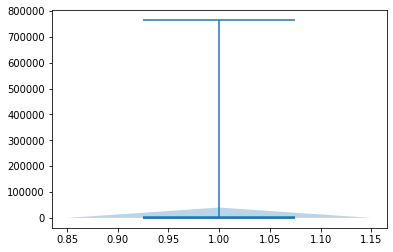
\includegraphics[width=\linewidth]{4_designing/figures/electricity_violin_unscaled.png}
        \caption{Unscaled violin plot of the electricity dataset}
        \label{fig:electricity_violin_unscaled}
    \endminipage\hfill
    \minipage{0.45\textwidth}
        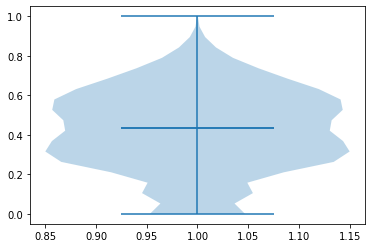
\includegraphics[width=\linewidth]{4_designing/figures/electricity_violin.png}
        \caption{Scaled violin plot of the electricity dataset where all timeseries have been scaled by their maximum value.}
        \label{fig:electricity_violin_scaled}
    \endminipage\hfill
\end{figure}


Another common tool for visualising timeseries is to generate a histogram of the timeseries. However as the datasets available in GluonTS contains tens of thousands of timeseries, plotting each of these individually is unfeasible. Thus for each dataset I aggregate the timeseries values so that it can be be displayed in a single plot. Instead of generating histograms I choose to generate violin plots as these capture both the distribution of values just as histograms do as well as the median value and the interquartile range. However as each timeseries in a dataset is on its own scale, the aggregate violin plot becomes hard to read. By scaling each timeseries in the dataset by the maximum value of that timeseries before plotting it the violin plot becomes more easy to read.  

In addition to these visual tools I calculate the following statistics for each of the datasets in GluonTS:

\begin{itemize}
\item Mean value
\item Max value
\item Min value
\item Number of timeseries
\item Number of datapoints
\item Length of shortest timeseries
\item Length of longest timeseries
\item Strength of the trend (mean and standard deviation)
\item Strength of the seasonality (mean and standard deviation)
\end{itemize}

Simple metrics such as the maximum, mean and minimum values for a dataset are useful in order to get a high level overview of the dataset. Furthermore, simpler statistics such as these can identify possible issues which can surface further down the line. For example, the metric used when evaluating forecasting methods can become unstable for some values in the dataset. One such example is the MAPE metric, which become unstable for timeseries close to 0 \cite{hyndman_forecasting_3rd}. 

The number of timeseries are important for global models as these then have more data which they can learn across which can help to combat overfitting. The number of timeseries is however not important for local models as these are only impacted by the quality and length of each individual time series. Longer timeseries however, benefit forecasting models which can handle longer horizons \cite{makridakis_m4_2020}. For these reasons, the number of timeseries and the lengths of the shortest and longest timeseries are necessary metrics when comparing datasets. Optimally one would have both long timeseries and many series as this would benefit both global and local models, however this is not always possible.

In chapter \ref{sec:dataset_character} we dove into seasonality and trend and how these describe the stationarity of timeseries. The strength of the seasonality and the trend of a timeseries can be calculated by: TODO add the equation here \cite{hyndman_forecasting_3rd}. The trend and the seasonality X and Y in equation Z can be extracted through STL decomposition. In my case I used the STL method of the python Statsmodel package. In order to apply this to an entire dataset, the strengths need to be calculated for each individual timeseries. Thereafter, the average value and standard deviation is recorded. Complimentary datasets should exhibit different values of strength for trend and seasonality. Additionally, the variance of these strengths are important as a higher variance indicates that the timeseries within a dataset are very mixed regarding the strength of trend and seasonality. 

Four types of datasets could be identified as a representable subset of datasets:

\begin{enumerate}
\item One dataset with high trend and low seasonality
\item One dataset with low trend and high seasonality
\item One dataset with low trend and low seasonality
\item One dataset with high trend and high seasonality
\end{enumerate}
\label{dataset_criteria}

\subsubsection{Limitations}
The M4 dataset does not significantly differ when compared to the m3 dataset except for its size \cite{m3_vs_m4} due to this, and that the m3 dataset has been largely superseeded by the m4 dataset, the m3 dataset was early discarded as the dataset of choice for this comparison. 
Another set of datasets which are not going to be used is the, the NIPS datasets. This is due to them having had some postprocessing applied to them. As the exact post processing is not known, comparing any findings when training on these datasets with other papers becomes hard and introduces uncertainty. In order to avoid this, these datasets are not considered. 

\subsection{result}
The complete plots and statistics are available in the appendix as they were to numerous to be displayed here. However a summary of the extracted statistics is presented in XXX.

The strength of the trend and seasonality can be easily viewed by generating a heatmap of the values as can be seen in figure \ref{heatmap_strengths}. 

\begin{figure}[htb]
    \centering
    \minipage{0.48\textwidth}
        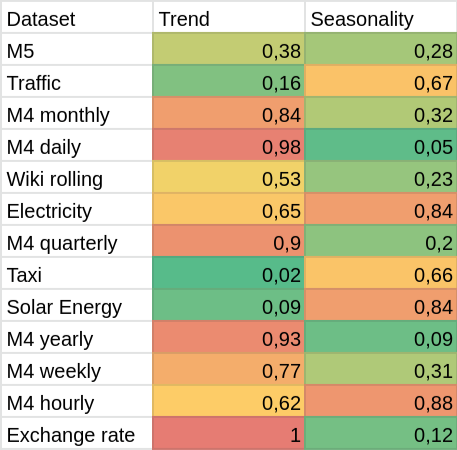
\includegraphics[width=\linewidth]{4_designing/figures/dataset_trend_seasonality_heatmap_mean.png}
        \caption{Heatmap of the strength of the trend and the seasonality sorted by the size of the datasets.}
    \endminipage\hfill
    \minipage{0.48\textwidth}
        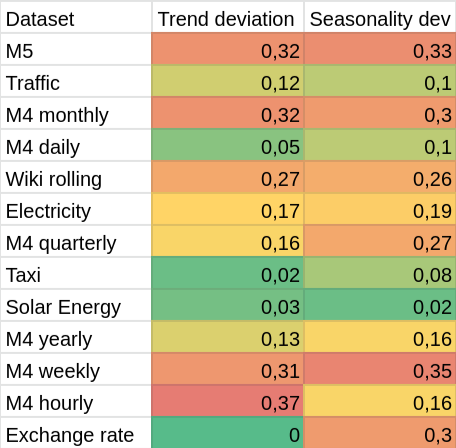
\includegraphics[width=\linewidth]{4_designing/figures/dataset_trend_seasonality_heatmap_deviation.png}
        \caption{Heatmap of the standard deviation of the strength of the trend and the seasonality for the datasets.}
    \endminipage\hfill
\end{figure}
\label{heatmap_strengths}

There is only one dataset in \ref{heatmap_strengths} which exhibits low trend and low seasonality and that is the m5 dataset. However the m5 dataset does show the most variance of all the datasets which implies that it contains many timeseries with and without trend and seasonality. 

In order to choose a dataset which fits into the category of high seasonality and low trend there are three options; Solar Energy, Taxi and Traffic. Of these the Solar Energy dataset has the lowest variance for both the trend and the seasonality. Further the solar energy dataset shows the highest seasonality of them all. 

The datasets with the lowest seasonality and the highest trends are the m4 datasets except for the m4 hourly and the Exchange rate dataset. Of these the one with the lowest variance as well as the highest trend is the Exchange Rate dataset closely followed by the m4 daily dataset. The size of the Exchange Rate dataset is much smaller than the m4 Daily dataset, with only 8 timeseries and 48k datapoints in comparison to the 4227 series and 9.9M datapoints.

When it comes to finding a dataset which both has a high trend and a high seasonality, there are only two options, the Electricity dataset and the m4 hourly dataset. They both have a high variance, however the variance of the Electricity dataset is slightly lower than that of m4 hourly. In addition, the Electricity dataset has almost twice the amount of datapoints as m4 hourly.

To summarize the four datasets which most closely fit the criteria defined in \ref{dataset_criteria} are:

\begin{table}[htp]
    \centering
    \begin{tabular}{ccc} % ccc means 3 columns, all centered; alternatives are l, r
                                & {\bf Low trend }  & {\bf High Trend}\\
        \hline % draws a line under the column headers
        {\bf Low seasonality}   & M5                & m4 daily\\
        \hline
        {\bf High Seasonality}  & Solar Energy      & Electricity\\
    \end{tabular}
    \caption{Datasets with complimentary strength of trend and strength of seasonality}
    \label{fig:representative_subset_of_datasets}
\end{table}

\section{Compairing statistical tests for reproducibility}
\label{subsubsec:choosing-statistical-test}
In this section the tests are compared in order to answer the questions in \ref{subsec:distributions}. Each of the tests are executed on data collected over 300 runs of DeepAR for three different hyperparameter configurations on the Electricity dataset \ref{fig:deepar_elec_300_hist}. Thus the statistical tests will be evaluated on in total 900 datapoints. In statistical tests are compared across a couple of different criteria.  

\begin{itemize}
    \item Can it accurately identify that two sets of samples are from the same distribution when one of the sets is small.
    \item Does it have a high false error rate, i.e. does it often mistake to identify samples from the same distribution. 
    \item Does it accurately detect when two distributions has different shape.
    \item How sensitive is it, i.e. can it detect differences in visually similar distributions.
\end{itemize}

\subsection{Methodology}

\subsection{Results}
\begin{figure}[htb]
    \centering
    \minipage{0.32\textwidth}
      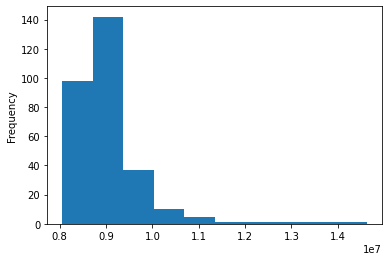
\includegraphics[width=\linewidth]{3_approach/figures/histogram_deepar_electricity_statistics_300_samples.png}
      \caption{Student-T}
      \label{fig:deepar_student_t_distibution}
    \endminipage\hfill
    \minipage{0.32\textwidth}
      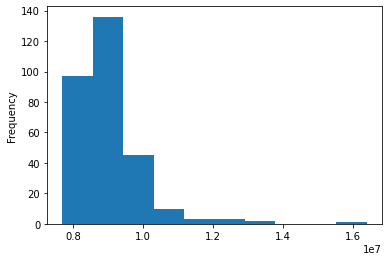
\includegraphics[width=\linewidth]{3_approach/figures/histogram_deepar_negbin_electricity_statistics_200_samples.png}
      \caption{Neg-Binomial}
      \label{fig:deepar_negbinomial_distibution}
    \endminipage\hfill
    \minipage{0.32\textwidth}%
      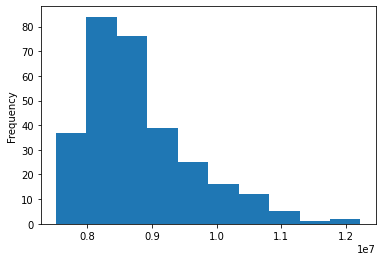
\includegraphics[width=\linewidth]{3_approach/figures/histogram_deepar_poisson_electricity_statistics_200_samples.png}
      \caption{Poisson}
      \label{fig:deepar_poisson_distribution}
    \endminipage
  \caption{\textbf{Histograms of the absolute error for 300 runs of DeepAR on the Electricity dataset} The three plots are generated through 300 runs of DeepAR on the Electricity dataset with three different values of the hyperparameter \emph{distr\_output} see section \ref{algo:deepar} for more info }
  \label{fig:deepar_elec_300_hist}
\end{figure}

As can be seen in \ref{fig:deepar_elec_300_hist} the distribution of the absolute error is skewed and more closely reflects a lognormal distribution than a normal distribution. This contradicts the key assumption made for the T-Test, Welch-s T-test and the naive approach. However as will be shown, these still perform well in the scenarios we consider below. 

TODO write this using some neat mathematical notation.
Given a small sample N, how does the different methods compare when evaluating if the sample is from the same distribution of another larger sample M? To answer this, I ran each test 297 times (0 <= |M| < 300 - |N|). N contained the 3 data points not in M. M contained {0, 1, ..., 297} samples of the 300 runs.  The results are presented in \ref{fig:false_positives}.

\begin{table}[htp]
    \centering
    \begin{tabular}{lcccc} % ccc means 3 columns, all centered; alternatives are l, r
        {\bf Name} & {\bf Errors} & {\bf \%} & {\bf Runs} & {\bf configuration}\\
        \hline % draws a line under the column headers
        Naive               & 52 & 17\% & 297 & negative binomial\\
        Naive               & 62 & 20\% & 297 & student t\\
        Naive               & 47 & 15\% & 297 & poisson\\
        \hline
        T-Test              & 24 & 8\%  & 297 & negative binomial\\
        T-Test              & 19 & 6\%  & 297 & student t\\
        T-Test              &  4 & 1\%  & 297 & poisson\\
        \hline
        Welchs T-Test       & 43 & 14\%  & 297 & negative binomial\\
        Welchs T-Test       & 39 & 13\%  & 297 & student t\\
        Welchs T-Test       &  23 & 7\%  & 297 & poisson\\
        \hline
        Kolmogorv-Smirnov   & 15 & 5\%  & 297 & negative binomial\\
        Kolmogorv-Smirnov   & 18 & 6\%  & 297 & student t\\
        Kolmogorv-Smirnov   & 3 & 1\%  & 297 & poisson\\
        \hline
        
    
    \end{tabular}
    \caption{\textbf{False positive rates of statistical tests for one small sample and one larger}}
    \label{fig:false_positives}
\end{table}

As can be seen in \ref{fig:false_positives} the naive approach have a higher error rate, i.e. it reports that the two distributions are sampled from different distributions more often when compared to the other approaches. The Kolmogorov Smirnov statistic performs the best with the lowest amount of errors out of all the tests. 

Calculating the general false positive rates is done similarly as above, however instead of fixing the size of \emph{N}, it will contain random samples of the remainder after \emph{M} is sampled from the 300 datapoints. I.e. tests will be applied for all combinations of samples where 0 < |\emph{M}| < 300 and 0 < |\emph{N}| < 300-|\emph{M}|


\begin{table}[htp]
    \centering
    \begin{tabular}{lcccc} % ccc means 3 columns, all centered; alternatives are l, r
        {\bf Name} & {\bf Errors} & {\bf \%} & {\bf Runs} & {\bf configuration}\\
        \hline % draws a line under the column headers
        Naive               & 241 & <1\% & 106900 & negative binomial\\
        Naive               & 313 & <1\% & 106900 & student t\\
        Naive               & 366 & <1\% & 106900 & poisson\\
        \hline
        T-Test              & 5489 & 5\%  & 106900 & negative binomial\\
        T-Test              & 5893 & 5\%  & 106900 & student t\\
        T-Test              & 34869 & 32\%  & 106900 & poisson\\
        \hline
        Welchs T-Test       & 12334 & 11\%  & 106900 & negative binomial\\
        Welchs T-Test       & 9037 & 8\%  & 106900 & student t\\
        Welchs T-Test       & 33971 & 31\%  & 106900 & poisson\\
        \hline
        Kolmogorv-Smirnov   & 4250 & 3\%  & 106900 & negative binomial\\
        Kolmogorv-Smirnov   & 5658 & 5\%  & 106900 & student t\\
        Kolmogorv-Smirnov   & 23417 & 21\%  & 106900 & poisson\\
        \hline
        
    
    \end{tabular}
    \caption[False positive rates of statistical tests]{\textbf{False positive rates of statistical tests}}
    \label{fig:false_positives}
\end{table}
